Due to some technical issues, we had to reset our EC2 instance, thus the findings presented are those collected following the reset. As of the writing of this paper, we have received over 1,300 attacks on our honeypots. Modern Honeypot Network provides some useful high level statistics about our honeypots some of which may be seen in Table 1 and Table 2. Another interesting observation is that the vast majority of our data came from Snort, as over 1,200 attacks originated on our Snort honeypot.

We also found that 1433 was attacked significantly than any other port. This is likely due to port 1433's use as the default port for many SQL servers.


\begin{table}[H]
	\resizebox{\columnwidth}{!}{%
	\begin{tabular}{|c|c|c|}
		\hline
		IP Address (first 5 digits) & Country     & Number of attacks \\ \hline
		45.136                 & Germany     & 21                \\ \hline
		80.82.7                & Netherlands & 18                \\ \hline
		83.97.2                & Romania     & 17                \\ \hline
		89.248                 & Netherlands & 17                \\ \hline
		81.22.4                & Russia      & 16                \\ \hline
	\end{tabular}%
	}
\caption{Top Five Individual Detected IP Addresses} \label{tab:ips}
\end{table}

\begin{table}[H]
	\resizebox{\columnwidth}{!}{%
	\begin{tabular}{|c|c|c|}
		\hline
		Attacked Port & Number of Attacks & Common Port Use                                                                               \\ \hline
		1433          & 195               & SQL Server                                                                                    \\ \hline
		22            & 70                & SSH                                                                                           \\ \hline
		5060          & 68                & Clear Text SIP, VoIP                                                                          \\ \hline
		445           & 18                & Server Message Block                                                                          \\ \hline
		8545          & 17                & \begin{tabular}[c]{@{}c@{}}Remote Procedure Call interface\\ of Ethereum clients\end{tabular} \\ \hline
	\end{tabular}%
	}
\caption{Top Five Attacked Ports} \label{tab:ports}
\end{table}

Using the \href{https://github.com/pieqq/PyGeoIpMap}{PyGeoIpMap} library, we were also able to plot the approximate locations of attacker IP addresses (Figure 1). Additionally, we plotted the top 20 countries by attacker, as seen in Figure 2. While IP addresses from all around the world were detected, the majority came from the United States, the Netherlands, China, Russia, and Germany. One note of importance regarding IP addresses is that the addresses we've encountered are not necessarily those of the attacker since attackers could be using VPNs.

\begin{figure}[H]
	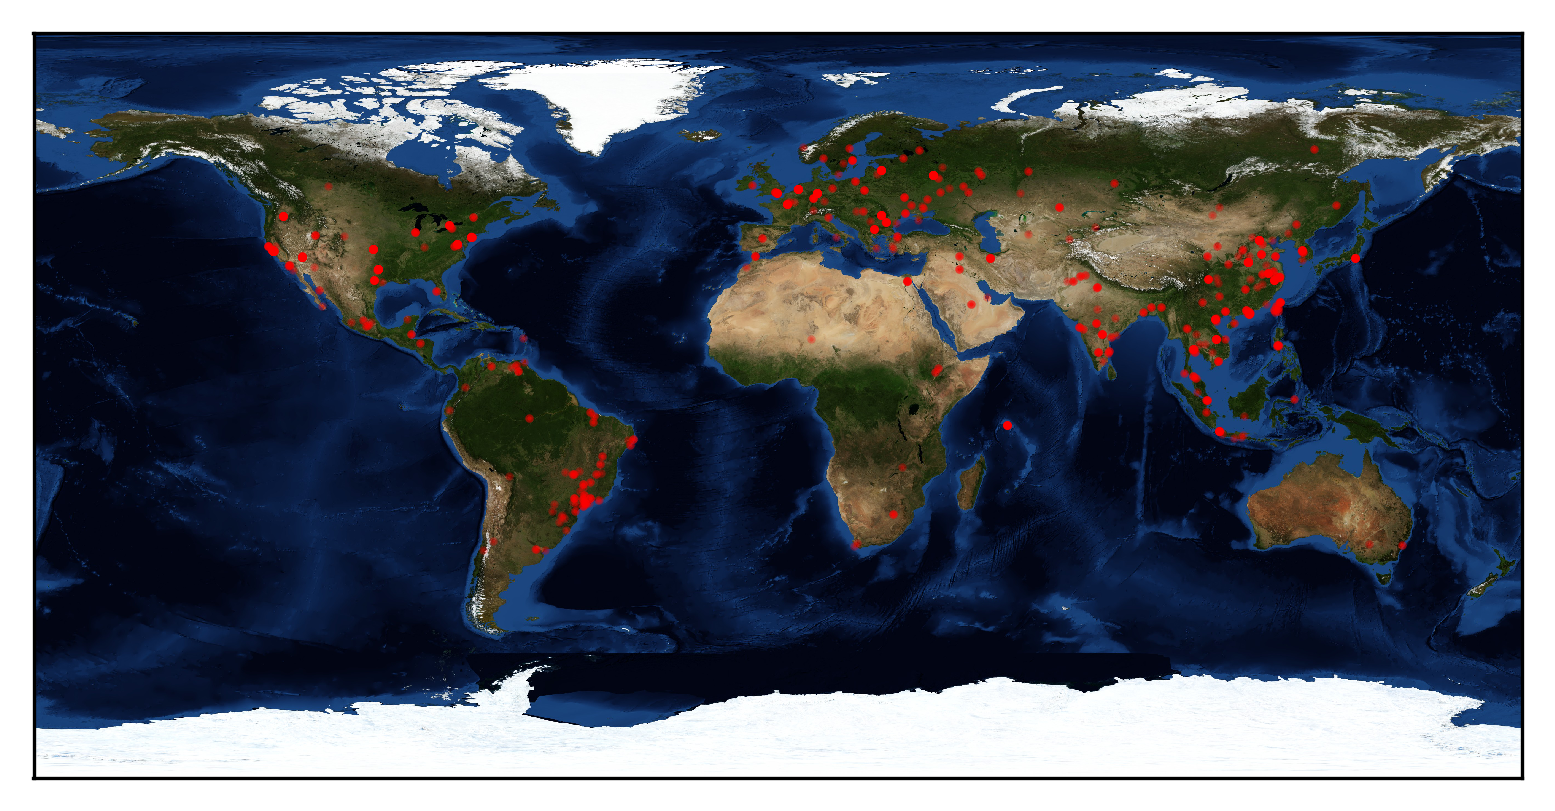
\includegraphics[width=\linewidth]{output.png}
	\caption{Approximate Locations of Attacker IP Addresses.}
	\label{fig:map}
\end{figure}


\begin{figure}[H]
	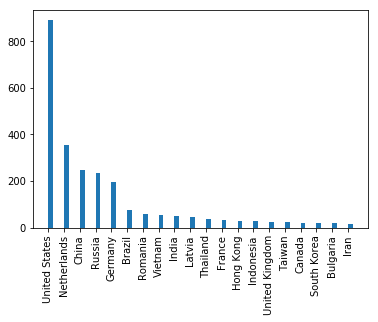
\includegraphics[width=\linewidth]{countries.png}
	\caption{Top Countries by Attacker.}
	\label{fig:top-countries}
\end{figure}
